\documentclass[12pt,oneside]{book}
\usepackage{geometry}                		
\geometry{a4paper}                   			
    		
\usepackage{graphicx}				
									
\usepackage{amssymb}

\usepackage[spanish]{babel}			
\usepackage[utf8]{inputenc}			
\usepackage[T1]{fontenc}				
\usepackage{hyperref}				



\title{Manual Haskell }
\author{Denisse Pintado}


						

\begin{document}
\maketitle
\tableofcontents

\chapter{Introducción}
En este proyecto se parsea documentos hechos en xml. El programa será realizado en el lenguaje puramente funcional Haskell. Este lenguaje tiene como característica fundamental la inclusión para soporte de tipos de datos y funciones recursivas. El proyecto deberá leer un archivo xml desde una dirección x, deberá ser cargado a memoria y leído línea por línea para poder procesar el documento por partes pequeñas, una vez hecho esto se pide identificar los tags de un documento xml teniendo en cuenta su estructura jerárquica, y poder leer los nombres y los atributos de los mismos. Haskell tienen librerías que ayudan a procesar los documentos xml, algo parecido al DOM en java, pero para fines académicos se deberá realizar la lectura por otros medios.
 \newpage
El proyecto de parsear un xml, nos ayuda a entender como trabaja Haskell, pudiendo describir comportamientos de lenguajes o de sistemas más complejos. El trabajo fue pensado para que se lean las estructuras del xml tomando en cuenta la jerarquía que existe en los tags o nodos de un archivo como este, y la relación de tienen los mismos a su vez. El método de lectura de archivos puede variar dependiendo de la forma como se piense solucionar la lectura, en este proyecto toma la asociación de poner un tag dentro de otro para  poder asociar el concepto de dependencia del documento. No se pudo implementar todas las consultas que se habían propuesto como es “Cuantos devices tienen true en cierta propiedad de los atributos de capability ”.Se tomó en cuenta las propiedades de todos los atributos de los tags y se pudo hacer consultas sencillas en base a esta estructura.

\begin{figure}
  \centering
    
\includegraphics[width=0.5\textwidth]{logohaskell.png}
  \caption{Haskell}
  \label{fig:logohaskell}
\end{figure}

\chapter{Alcance}

El proyecto lee los nodos del documento y el contenido de los mismos, así como el nombre de los atributos y el valor, genera una lista de la lectura y da la opción de consultar información que el documento tiene encriptado.


\begin{figure}
  \centering
    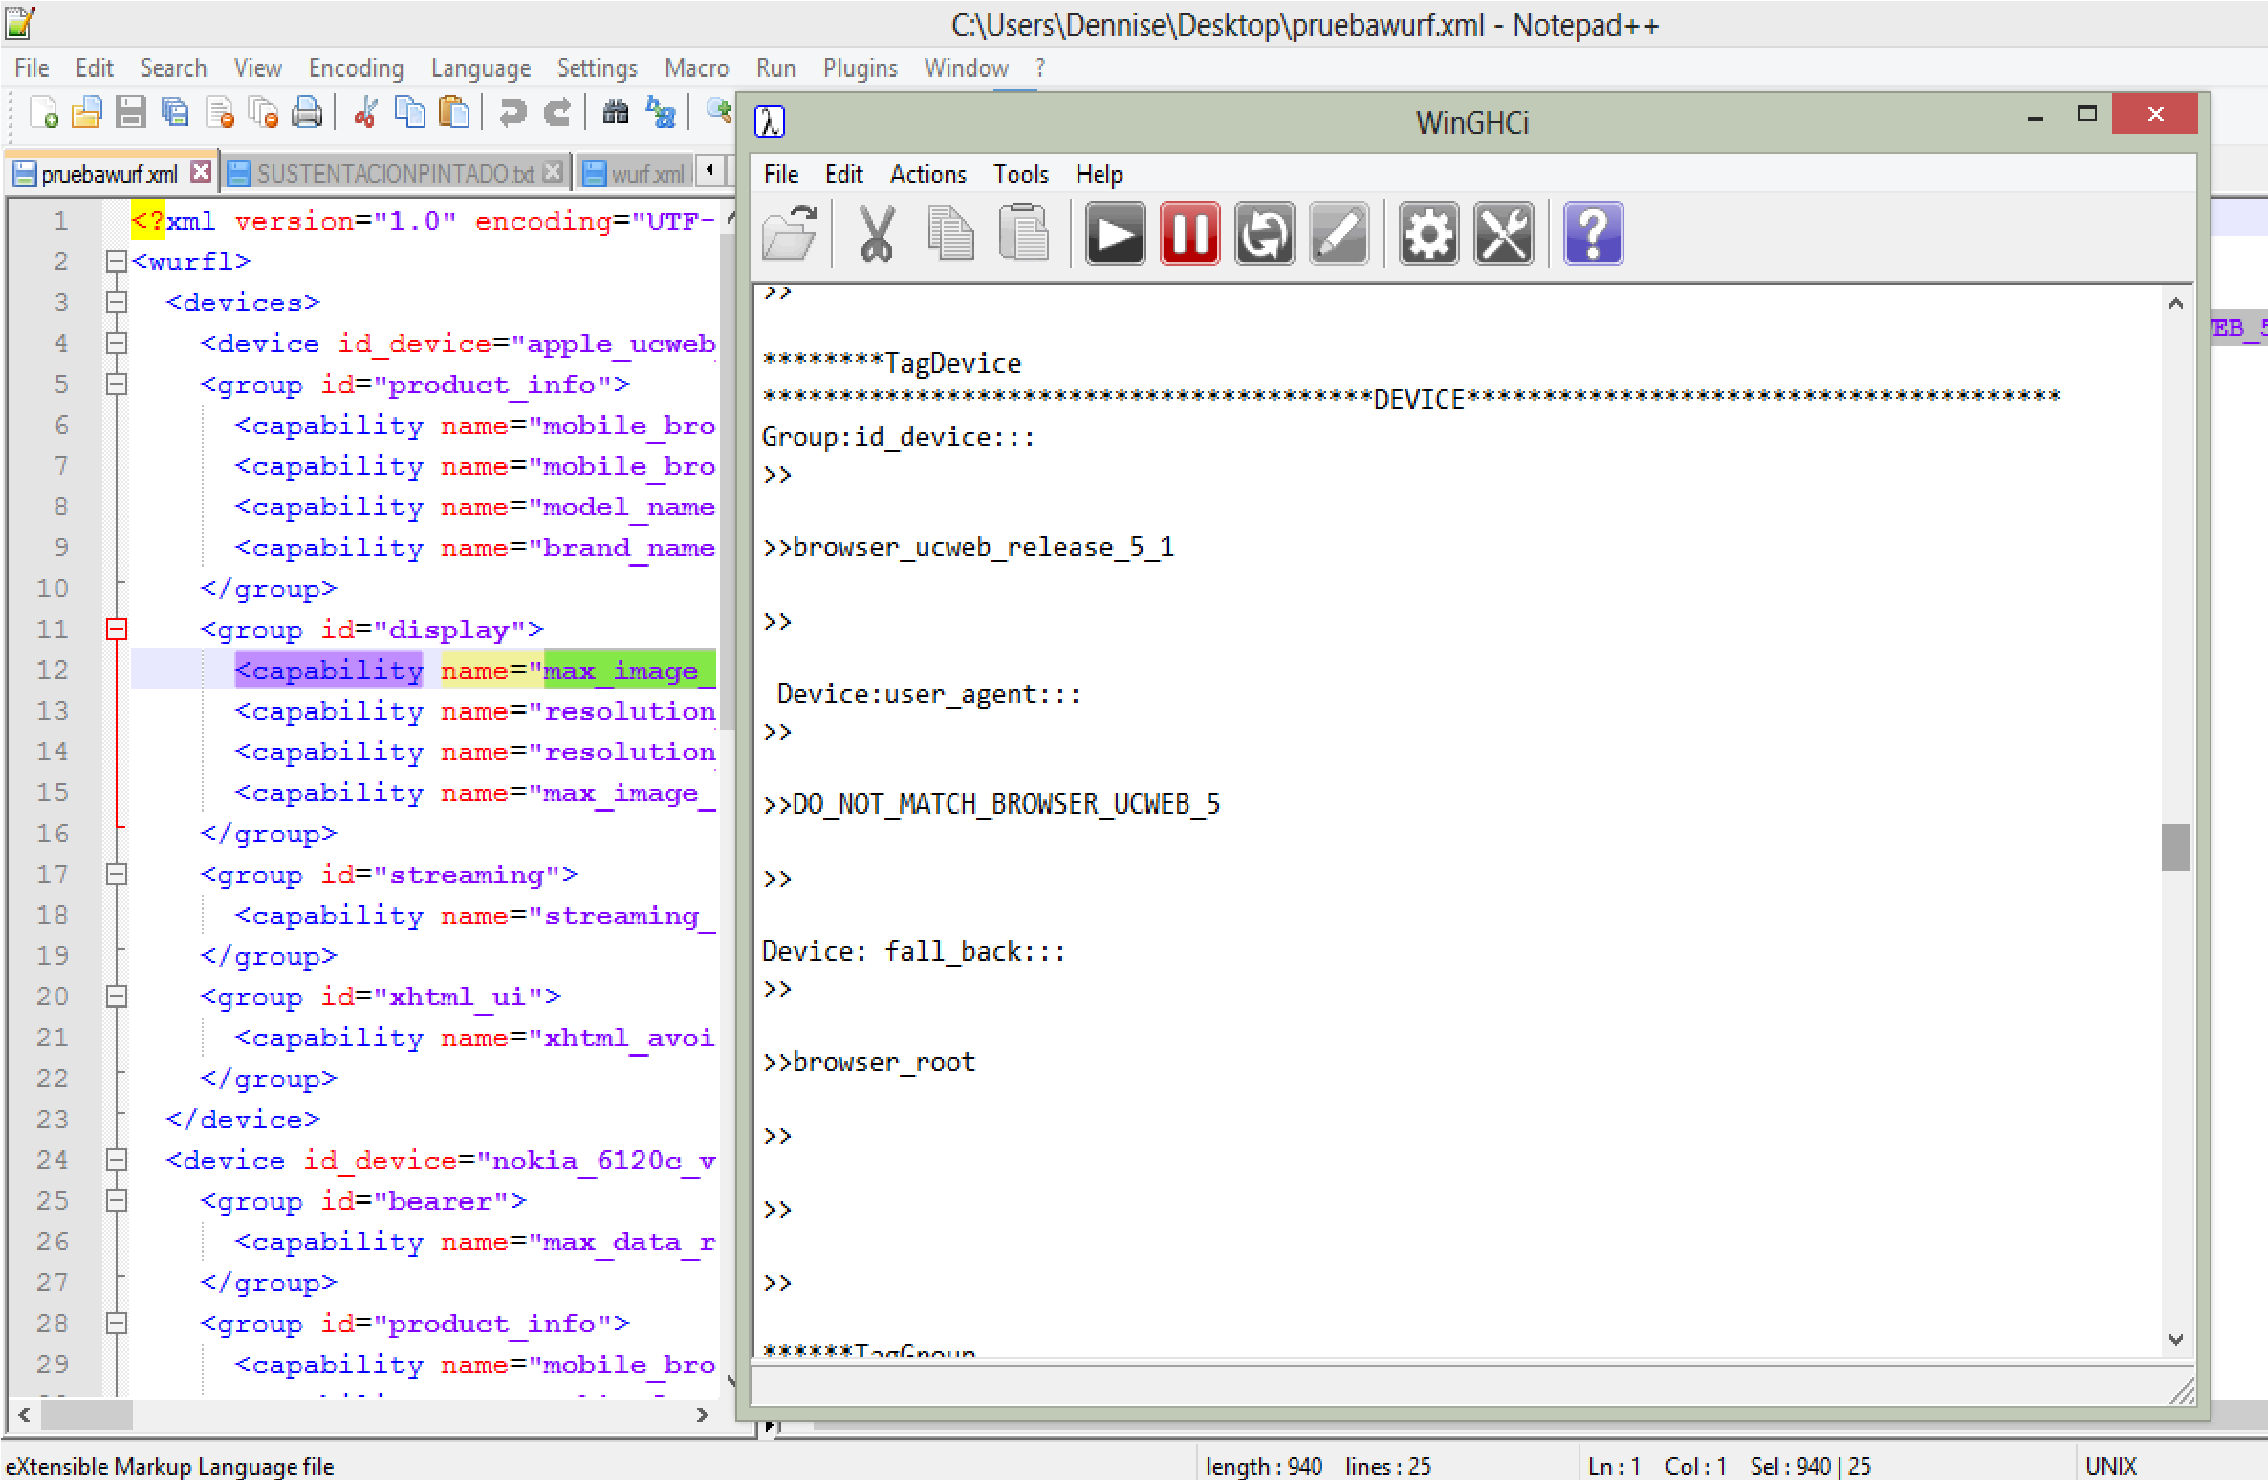
\includegraphics[width=0.5\textwidth]{capturaHaskell1.png}
  \caption{Funcionalidad}
  \label{fig:logohaskell}
\end{figure}


\chapter{Conclusiones}
Se pudo lograr lo que se defino al comienzo del proyecto. El programa resulto un poco complicado por la manera recursiva que trata toda función. Además resulto difícil personalmente tratar de simplificar pasos para que todo se haga en resumidas líneas a pesar de que se supone que el lenguaje esta diseñado para hacer de funciones complicadas sencillas programaciones. Haskell se asegura de que no haya efecto secundario y esto da poca versatilidad al momento de programar el codgio.

\chapter{Bibliografía}

https://github.com/jnunemaker/crack

http://www.haskell.org/haskellwiki/HXT

https://www.fpcomplete.com/school/starting-with-haskell/libraries-and-frameworks

https://github.com/josanvel/AnalizadorSintacticoXML

http://fileadmin.cs.lth.se/cs/Education/EDAN40/assignment4/parser.pdf

http://www.fceia.unr.edu.ar/lcc/t321/archivos/11.ALPII.Clase09.Parsers.pdf

http://www.fh-wedel.de/~si/HXmlToolbox/cookbook/doc/thesis.pdf

http://en.wikibooks.org/wiki/Haskell/XML

\end{document}  
